\section{Analysis and Discussion}
\label{section_7}

% \begin{table}[t]
% \caption{Performance Comparison of Different Speculative Decodings.}
% \centering
% \includegraphics[width=\colimgwidth]{Tables/6_5_Speculative_Decoding_Comparison.pdf}
% \label{table_6_3}
% \vspace{-0.20in}
% \end{table}


\subsection{Cassandra and Quantization: From Performance Rivalry to Algorithmic Synergy}
\label{section_7_1}
Quantization has emerged as a critical methodology for optimizing LLM inference performance. In particular, high-bit quantization formats, such as INT8, FP8 and MXFP8, are widely recognized for their robustness; this may raise questions regarding the necessity of lossless acceleration techniques like Cassandra. Nevertheless, Cassandra offers distinct advantages over the mere employment of high-bit quantization.

\subsubsection{Unpredictable Accuracy Degradation in Quantization}
According to previous studies~\cite{Quantization-Hurts-Reasoning, llama70b-quant, llama405b-quant}, even quantization techniques generally known to maintain accuracy can suffer from significant performance degradation under specific conditions. For instance, applying W8A8 SmoothQuant~\cite{Smoothquant} to Llama3.1-405B results in an average accuracy decline of 10.86\% across the OpenLLM Leaderboard-v2 datasets~\cite{llama405b-quant}. Such unpredictable degradations manifest across a wide range of model scales, from Qwen2.5-1.7B to Llama3.1-405B. Furthermore, quantization alters the model's probability distribution, potentially leading to unpredictable behaviors. For instance, a study~\cite{Accuracy-is-Not-All-You-Need} reported that applying W8A16 GPTQ~\cite{GPTQ} to Qwen2-1.5B~\cite{Qwen2-1.5B} resulted in only a 0.3\% accuracy drop on the GSM8K benchmark~\cite{GSM8K}; however, 6.37\% of the actual predicted answers changed compared to the original model.

For these reasons, despite the high efficiency of quantization, there remains a strong demand for lossless LLM inference acceleration, where speculative decoding is often employed independently without quantization. Furthermore, recent studies~\cite{dfloat11, LILO, Zipserv} have begun exploring the use of lossless compression techniques to accelerate LLM inference, without relying on speculative decoding.

\subsubsection{Performance Superiority of Cassandra in Low-Batch Inference}
Figure~\ref{fig_6_1} shows that Cassandra achieves up to a 2.41x speedup compared to the BFloat16 baseline. In contrast, 8-bit quantization yields only a 1.3$\times$ performance improvement over BFloat16. The observed performance degradation stems from the overhead associated with online activation quantization and scaling factor multiplication. In the prefill stage, where GEMM execution time is the main bottleneck, this overhead is largely masked by the gains from reduced GEMM computation. However, in low-batch LLM inference, the decode stage accounts for the majority of the end-to-end latency. Since GEMM is not the bottleneck in the decode stage, the overhead from activation quantization and scaling become non-negligible. Previous studies~\cite{Smoothquant, FP8-Quantization-Performance} have also reported that the decode stage performance of INT8 and FP8 quantization ranges from 1.25$\times$ to 1.42$\times$ compared to FP16 and BF16 baseline, which aligns with our measurements.

\subsubsection{Compatibility with Quantization}
While we utilize BFloat16 as our baseline, Cassandra is fully compatible with quantization. The most straightforward format to integrate into Cassandra is MXINT8. Currently, Cassandra-2 employs the MXINT format during the draft model generation process. Extending this approach to ensure the entire target model utilizes the MXINT8 format can be achieved seamlessly. According to prior research~\cite{INT-vs-FP}, MXINT8 exhibits overhead similar to other 8-bit quantization methods and generally offers superior accuracy compared to MXFP8.

Furthermore, with minor modifications, Cassandra can be extended to INT precision. Any-precision LLM~\cite{Any-Precision-LLM} serves as an excellent example of INT quantization that can be integrated with Cassandra. These methods propose multi-precision quantization techniques that allow for the deployment of optimized lower-bit models via simple truncation, which aligns perfectly with Cassandra’s core algorithm of generating draft models through pruning and truncation.





\subsection{Comparison with Other Speculative Decoding Methods}
\label{section_7_2}

\begin{figure}[t]
\centering
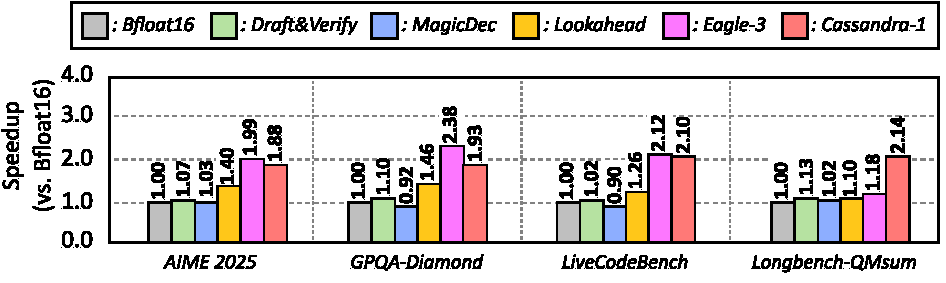
\includegraphics[width=\colimgwidth]{Figures/6_6_speculative_decoding_performance.pdf}
\caption{Performance Comparison of Different Speculative Decodings.}
\label{fig_7_1}
\vspace{-1.5em}
\end{figure}


\subsubsection{Performance}

Figure~\ref{fig_7_1} illustrates the performance improvements of various speculative decoding schemes relative to the BFloat16 baseline. For our evaluation, we employed Draft\&Verify~\cite{Draft&Verify}, MagicDec~\cite{MagicDec}, and Lookahead Decoding~\cite{Lookahead-Decoding} as representative training-free speculative decoding methods, while EAGLE-3~\cite{eagle3} was utilized as the training-based speculative decoding baseline. All experiments were conducted using official open-source implementations. Also, we utilized DeepSeek-distill-Llama-8B~\cite{Deepseek-R1-Distillated-Llama3-8B} to leverage the official EAGLE-3 draft weights. Furthermore, since all speculative decoding frameworks utilize a BFloat16 target model, we selected Cassandra-1 as our baseline to ensure a fair comparison.

As shown in Figure~\ref{fig_7_1}, Cassandra consistently outperforms Draft\&Verify, MagicDec, and Lookahead Decoding across all four benchmarks. In the case of MagicDec, its reliance on KV cache pruning leads to significantly degraded performance in low-batch inference scenarios, occasionally even performing slower than the baseline.

Draft\&Verify also fails to generate a efficient draft model through its Bayesian-based layer skipping; although it skips 18 attention layers from the original 32-block model, it only skips 9 FFN layers. Consequently, the draft model must still load 70.7\% of the original model's parameters, a structure that is fundamentally limited in achieving high-speed execution for low-batch LLM inference.

Regarding Lookahead Decoding, which predicts subsequent tokens by referencing N-gram sets generated from previous data, it exhibited lower performance gains compared to Cassandra, particularly on LongBench and LiveCodeBench. Nevertheless, it achieved notable speedups of 1.40$\times$ and 1.46$\times$ on AIME2025 and GPQA-Diamond, respectively.

While EAGLE-3 demonstrated superior performance over Cassandra on AIME2025 and GPQA-Diamond, its effectiveness is heavily biased toward the characteristics of its training data. As illustrated, EAGLE-3 shows a significantly diminished margin of improvement in specific tasks such as long-sequence understanding. These results confirm that Cassandra not only outperforms most existing speculative decoding schemes across diverse scenarios but also provides robust performance gains with minimal sensitivity to sequence length or task type.

\subsubsection{Pre-Computation Cost}

To utilize Cassandra, two distinct pre-computation steps are required. The first step involves calibration for Wanda-based weight pruning. A small calibration set of approximately 128 samples is sufficient for this pruning method to deliver robust performance~\cite{Wanda}. Other techniques employed in Cassandra, such as exponent compression, KV cache pruning, and mantissa truncation, do not require any calibration. The second step is the optimization of ratio for pruning and truncation. The optimal combination of pruning ratio and truncation bits for configuring the draft model can be determined based on the acceptance rate relative to the compression ratio, which can be expressed by the following objective function.

\begin{equation}
\text{\small} % 또는 \footnotesize
\mathcal{J} = \frac{\alpha}{S_w(1 - w_p)(B - w_t) + S_{kv}(1 - kv_p)(B - kv_t)}
\end{equation}
\vspace{0.03in}

Here, $S_w$ denotes the weight size, $S_{kv}$ is the KV cache size, $w_t$ and $kv_t$ represent the truncation bits for weights and the KV cache respectively, $w_p$ and $kv_p$ are the pruning ratios for weights and the KV cache, $B$ is the number of bits used by the target model, and $\alpha$ is the acceptance rate.

As a practical approach to identifying a local optimum, we recommend prioritizing the optimization of hyperparameters associated with the dominant term by comparing the magnitudes of $S_w$ and $S_{kv}$. We conducted a grid search by incrementing the pruning ratio for weights and KV cache from 30\% to 60\% in 10\% intervals and the truncation range from 0 to 5 bits in 1 bit intervals. Following the experimental setup of Draft\&Verify, we used a development set of 8 samples. When using an 8B model, this process requires approximately 5 minutes of GPU time on an NVIDIA A100. In comparison with competing approaches, this overhead is acceptable; for instance, Eagle-3 requires 96 to 192 GPU hours on an A100, and Draft\&Verify requires approximately 1.5 hours of Bayesian optimization on A100 for an 8B model.

% Furthermore, considering that Lookahead Decoding needs re-tuning the window size, N-gram size, and candidate number based on the GPU and model scale, Cassandra is highly economical compared to other speculative decoding frameworks.

Additionally, unlike other hyperparameters that vary drastically across models, our default configuration, a 40\% pruning ratio and 4 bit truncation, demonstrates robust transferability to other models. Users can either adopt this configuration directly or use it as a starting point to narrow the search space, further reducing the cost of finding a local optimal solution.





\begin{figure}[t]
\centering
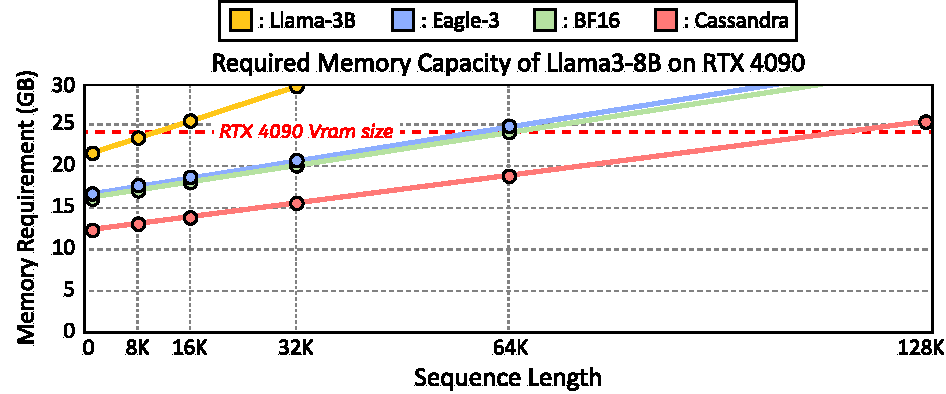
\includegraphics[width=\colimgwidth]{Figures/6_5_Memory_Capacity.pdf}
\caption{Comparison of memory requirements between autoregressive decoding and various speculative decoding methods.}
\label{fig_6_3}
\vspace{-1.5em}
\end{figure}

\subsubsection{Memory Capacity Requirement}
Figure~\ref{fig_6_3} shows the ideal memory capacity requirement in various decoding schemes. As shown in the figure, Cassandra exhibits the most superior memory capacity efficiency compared to other speculative decoding methods and can generate 11.59$\times$ and 1.81$\times$ more tokens than Llama3-based speculative decoding and Eagle-3, respectively. Due to its exponent compression and memory-efficient draft model design, Cassandra actually requires less memory capacity than the original BFloat16 format. This is yet another reason why Cassandra is suitable for resource-constrained devices.







% Figure~\ref{fig_7_1} presents the performance improvement of different speculative decoding schemes relative to BFloat16 when executing the AIME2025~\cite{AIME2025} and Longbench-QMSum~\cite{Longbench} benchmarks on DeepSeek-R1-Distillated-Llama-8B. For a fair comparison, we also re-measured the performance improvement of the other speculative decoding methods using our simulator, which yielded a higher value than the performance improvement obtained on the real GPU.

% As shown in Figure~\ref{fig_7_1}, Cassandra-1 demonstrates superior performance by a large margin compared to training-free speculative decoding methods, and even shows better performance in Longbench-QMSUM compared to Eagle-3. We confirmed that Eagle-3 also exhibits a throughput improvement of more than 4$\times$ in specific benchmarks. However, we found that Eagle-3's performance is highly sensitive to changes in prompts and tasks, and it shows particularly limited performance improvements in long sequences. Draft\&Verify achieved a high acceptance rate in an environment where 18 attention layers and 9 FFN layers were skipped. In this case, the draft model used in Draft\&Verify actually exhibits a very limited compression ratio, making it difficult to achieve significant performance improvement, particularly in single batch, short sequence environments where the FFN accounts for a large portion of the latency. MagicDec, which focuses on KV cache quantization, also showed only limited performance improvements in single-batch environments.


% Based on the AIME2025 benchmark, Cassandra outperforms traditional self-speculative decoding, but falls short when compared to Eagle-3. However, Cassandra is a training-free solution, yet it shows a superior performance gain compared to other training-free solutions.

% Furthermore, Cassandra demonstrates stronger performance than training-based speculative decoding in long-sequence inference scenarios. We ran both Eagle-3 and Cassandra on the QMSum and counted the average number of accepted tokens. Cassandra was able to predict an average of 3.51 tokens, whereas Eagle-3 predicted only an average of 0.53 tokens. With such a low acceptance rate, Eagle-based methods can actually lead to performance degradation.

% This suggests that the approach used by Eagle-3 may not provide acceleration when performing tasks that handle relatively long sequences. This issue arises because draft models created via distillation are generally too small to understand long sequences and are also heavily influenced by the training data. In contrast, Cassandra generates the draft model from the original model, which was trained on a sufficient dataset, allowing it to maintain strong performance across a variety of these tasks.